\documentclass[a4paper,12pt]{article}

\setlength{\parskip}{\baselineskip} % Spacing between paragraphs
\setlength{\parindent}{0pt} % Don't indent new paragraphs

\usepackage{tikz}
\tikzset{
	treenode/.style = {align=center, inner sep=0pt, text centered,  font=\small},
	explored/.style = {treenode, circle, black, draw=black,  text width=1.2em},
	hid/.style = {treenode, circle, lightgray, dashed},
	pruned/.style = {treenode, circle, lightgray, dashed, draw=black, font=\sffamily\bfseries, text width=1.2em},
	expr/.style = {treenode, draw=black},
	dead/.style = {treenode, draw=black}
}

% Floating picture next to each other
\usepackage{floatrow}
\usepackage{subfig}
\floatsetup[figure]{style=plain,subcapbesideposition=center}


\begin{document}

\begin{figure}[!htbp]% h=here allowed, t=top, b=bottom, p=on a float-page
	\sidesubfloat[]{%
		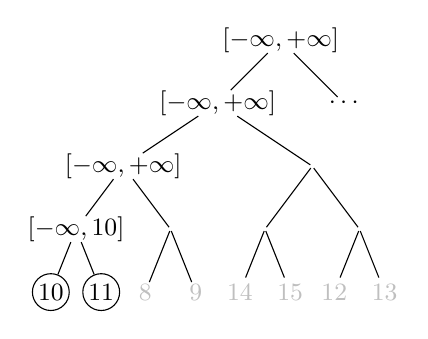
\begin{tikzpicture}[scale=0.8,
			level/.style={level distance=1cm},
		 	level 1/.style={sibling distance = 2cm},
		 	level 2/.style={sibling distance = 3cm},
		 	level 3/.style={sibling distance = 1.5cm},
		 	level 4/.style={sibling distance = 0.8cm}
		]
		\node [treenode] {[$-\infty, +\infty$]}
		child{ node [treenode] {[$-\infty, +\infty$]}
			child{ node [treenode] {[$-\infty, +\infty$]}
				child{ node [treenode] {[$-\infty, 10$]}
					child{ node [explored] {10}}
					child{ node [explored] {11}}
				}
				child{ node [treenode] {}
					child{ node [hid] {8}}
					child{ node [hid] {9}}
				}
			}
			child{ node [treenode] {}
				child{ node [treenode] {}
					child{ node [hid] {14}}
					child{ node [hid] {15}}
				}
				child{ node [treenode] {}
					child{ node [hid] {12}}
					child{ node [hid] {13}}
				}
			}
		}
		child{ node [treenode] {$\cdots$} }
		;
		\end{tikzpicture}
	}
	\qquad%
	\sidesubfloat[]{%
		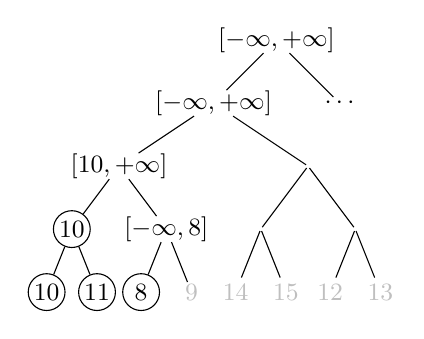
\begin{tikzpicture}[scale=0.8,
			level/.style={level distance=1cm},
		 	level 1/.style={sibling distance = 2cm},
		 	level 2/.style={sibling distance = 3cm},
		 	level 3/.style={sibling distance = 1.5cm},
		 	level 4/.style={sibling distance = 0.8cm}
		]
		\node [treenode] {[$-\infty,+\infty$]}
		child{ node [treenode] {[$-\infty, +\infty$]}
			child{ node [treenode] {[$10, +\infty$]}
				child{ node [explored] {10}
					child{ node [explored] {10}}
					child{ node [explored] {11}}
				}
				child{ node [treenode] {[$-\infty, 8$]}
					child{ node [explored] {8}}
					child{ node [hid] {9}}
				}
			}
			child{ node [treenode] {}
				child{ node [treenode] {}
					child{ node [hid] {14}}
					child{ node [hid] {15}}
				}
				child{ node [treenode] {}
					child{ node [hid] {12}}
					child{ node [hid] {13}}
				}
			}
		}
		child{ node [treenode] {$\cdots$} }
		;
		\end{tikzpicture}
	}
	\qquad%
	\bigbreak%
	\sidesubfloat[]{%
		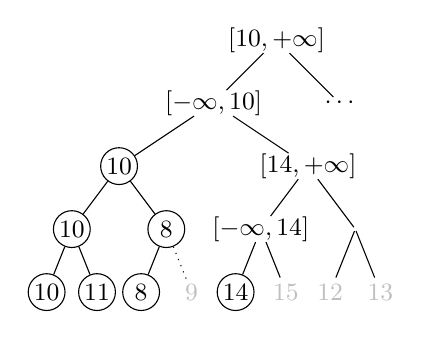
\begin{tikzpicture}[scale=0.8,
			level/.style={level distance=1cm},
		 	level 1/.style={sibling distance = 2cm},
		 	level 2/.style={sibling distance = 3cm},
		 	level 3/.style={sibling distance = 1.5cm},
		 	level 4/.style={sibling distance = 0.8cm}
		]
		\node [treenode] {[$10, +\infty$]}
		child{ node [treenode] {[$-\infty, 10$]}
			child{ node [explored] {10}
				child{ node [explored] {10}
					child{ node [explored] {10}}
					child{ node [explored] {11}}
				}
				child{ node [explored] {8}
					child{ node [explored] {8}}
					child[dotted]{ node [hid] {9}}
				}
			}
			child{ node [treenode] {[$14, +\infty$]}
				child{ node [treenode] {[$-\infty, 14$]}
					child{ node [explored] {14}}
					child{ node [hid] {15}}
				}
				child{ node [treenode] {}
					child{ node [hid] {12}}
					child{ node [hid] {13}}
				}
			}
		}
		child{ node [treenode] {$\cdots$} }
		;
		\end{tikzpicture}
	}
	\qquad%
	\sidesubfloat[]{%
		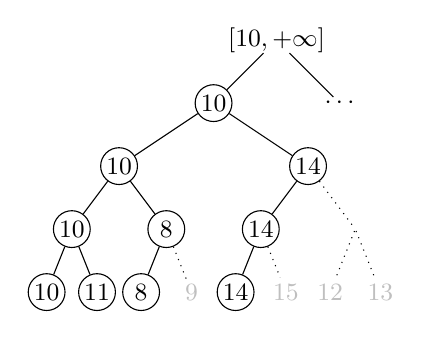
\begin{tikzpicture}[scale=0.8,
			level/.style={level distance=1cm},
		 	level 1/.style={sibling distance = 2cm},
		 	level 2/.style={sibling distance = 3cm},
		 	level 3/.style={sibling distance = 1.5cm},
		 	level 4/.style={sibling distance = 0.8cm}
		]
		\node [treenode] {[$10, +\infty$]}
		child{ node [explored] {10}
			child{ node [explored] {10}
				child{ node [explored] {10}
					child{ node [explored] {10}}
					child{ node [explored] {11}}
				}
				child{ node [explored] {8}
					child{ node [explored] {8}}
					child[dotted]{ node [hid] {9}}
				}
			}
			child{ node [explored] {14}
				child{ node [explored] {14}
					child{ node [explored] {14}}
					child[dotted]{ node [hid] {15}}
				}
				child[dotted]{ node [treenode] {}
					child{ node [hid] {12}}
					child{ node [hid] {13}}
				}
			}
		}
		child{ node [treenode] {$\cdots$} }
		;
		\end{tikzpicture}
	}
	\qquad%
	\bigbreak%
	\sidesubfloat[]{%
		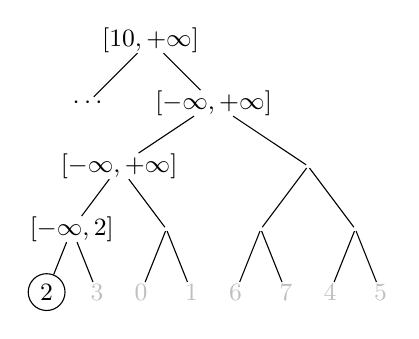
\begin{tikzpicture}[scale=0.8,
			level/.style={level distance=1cm},
		 	level 1/.style={sibling distance = 2cm},
		 	level 2/.style={sibling distance = 3cm},
		 	level 3/.style={sibling distance = 1.5cm},
		 	level 4/.style={sibling distance = 0.8cm}
		]
		\node [treenode] {[$10, +\infty$]}
		child{ node [treenode] {$\cdots$} }
		child{ node [treenode] {$[-\infty, +\infty]$}
			child{ node [treenode] {$[-\infty, +\infty]$}
				child{ node [treenode] {$[-\infty, 2]$}
					child{ node [explored] {2}}
					child{ node [hid] {3}}
				}
				child{ node [treenode] {}
					child{ node [hid] {0}}
					child{ node [hid] {1}}
				}
			}
			child{ node [treenode] {}
				child{ node [treenode] {}
					child{ node [hid] {6}}
					child{ node [hid] {7}}
				}
				child{ node [treenode] {}
					child{ node [hid] {4}}
					child{ node [hid] {5}}
				}
			}
		}
		;
		\end{tikzpicture}
	}
	\qquad%
	\sidesubfloat[]{%
		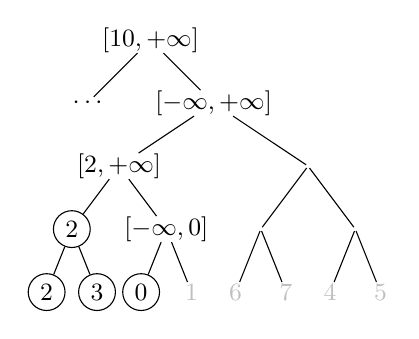
\begin{tikzpicture}[scale=0.8,
			level/.style={level distance=1cm},
		 	level 1/.style={sibling distance = 2cm},
		 	level 2/.style={sibling distance = 3cm},
		 	level 3/.style={sibling distance = 1.5cm},
		 	level 4/.style={sibling distance = 0.8cm}
		]
		\node [treenode] {[$10, +\infty$]}
		child{ node [treenode] {$\cdots$} }
		child{ node [treenode] {$[-\infty, +\infty]$}
			child{ node [treenode] {$[2, +\infty]$}
				child{ node [explored] {2}
					child{ node [explored] {2}}
					child{ node [explored] {3}}
				}
				child{ node [treenode] {$[-\infty, 0]$}
					child{ node [explored] {0}}
					child{ node [hid] {1}}
				}
			}
			child{ node [treenode] {}
				child{ node [treenode] {}
					child{ node [hid] {6}}
					child{ node [hid] {7}}
				}
				child{ node [treenode] {}
					child{ node [hid] {4}}
					child{ node [hid] {5}}
				}
			}
		}
		;
		\end{tikzpicture}
	}
	\qquad%
	\bigbreak%
	\sidesubfloat[]{%
		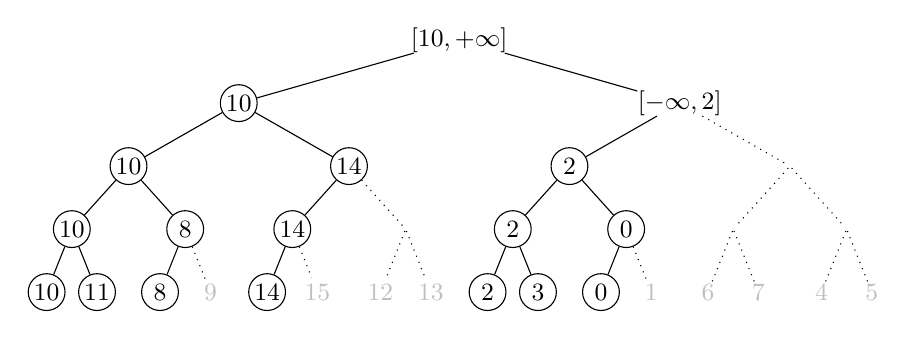
\begin{tikzpicture}[scale=0.8,
			level/.style={level distance=1cm},
		 	level 1/.style={sibling distance = 7cm},
		 	level 2/.style={sibling distance = 3.5cm},
		 	level 3/.style={sibling distance = 1.8cm},
		 	level 4/.style={sibling distance = 0.8cm}
		]
		\node [treenode] {[$10, +\infty$]}
		child{ node [explored] {10}
			child{ node [explored] {10}
				child{ node [explored] {10}
					child{ node [explored] {10}}
					child{ node [explored] {11}}
				}
				child{ node [explored] {8}
					child{ node [explored] {8}}
					child[dotted]{ node [hid] {9}}
				}
			}
			child{ node [explored] {14}
				child{ node [explored] {14}
					child{ node [explored] {14}}
					child[dotted]{ node [hid] {15}}
				}
				child[dotted]{ node [treenode] {}
					child{ node [hid] {12}}
					child{ node [hid] {13}}
				}
			}
		}
		child{ node [treenode] {$[-\infty, 2]$}
			child{ node [explored] {2}
				child{ node [explored] {2}
					child{ node [explored] {2}}
					child{ node [explored] {3}}
				}
				child{ node [explored] {0}
					child{ node [explored] {0}}
					child[dotted]{ node [hid] {1}}
				}
			}
			child[dotted]{ node [treenode] {}
				child{ node [treenode] {}
					child{ node [hid] {6}}
					child{ node [hid] {7}}
				}
				child{ node [treenode] {}
					child{ node [hid] {4}}
					child{ node [hid] {5}}
				}
			}
		}
		;
		\end{tikzpicture}
	}
	\caption{}
\end{figure}

Above is illustrated the process of the \emph{Aplha-Beta} pruning on the tree in Part (a). Note the grey numbers are \emph{to be} explored and the dotted lines are \emph{pruned} branches of the tree.

In Figure (a), just looking at the left side of the tree, the left most branch is explored first and a 10 is discover which is better than the current $\beta$ value of $-\infty$. The leaf node 11 is then explored.

In Figure (b) MIN chooses 10 and sets its parent $\alpha$ to this. The left most side of the next branch is explored to reveal an 8 which becomes the new $\beta$ of its parent MIN node. 

In Figure (c) the leaf node 9 gets pruned as the parent $\alpha$ (10) is greater than the child $\beta$ (8). Then leaf node 14 branch is explored.

In Figure (d) since the 2nd level MIN node has $\beta = 10$ thus the 14 will never be chosen by MIN so the 15, 12 and 13 branches are pruned.

In Figure (e) we switch over to the right hand side of the tree with the root nodes $\alpha$ set to 10. The 2 leaf node is explored  and its parent $\beta$ set to 2.

(f) The leaf node 3 is explored and the parent is set to 2 as a result of $MIN(2, 3)$. The parent MAX has its $\alpha$ set to 2. The leaf node 0 is explored and its parent $\beta$ set to 0.

(g) Since the 3rd level MAX has $\alpha = 2$ and its right child node's $beta = 2$, the leaf node 1 is pruned and the 2 propagated up the the parent MIN nodes $beta$. Since the root nodes $alpha$ (10) is greater than the MIN child's $beta$ (2), ensuring this will never be greater than 2, the root MAX will always choose the left 10 and the search terminates here.



\end{document}